% !TEX program = xelatex
\documentclass[UTF8,a4paper,zihao=-4,fontset=fandol]{ctexart}
\usepackage[margin=2.3cm]{geometry}
\usepackage{amsmath,amssymb,booktabs,longtable,graphicx,float,tabularx}
\usepackage{xcolor,tikz,fancyhdr,hyperref,caption}
\usepackage{xurl}
\usetikzlibrary{arrows.meta,positioning}
\hypersetup{colorlinks=true,linkcolor=black,urlcolor=blue,citecolor=black,pdftitle={微网储能与购电调控策略：第二版研究稿}}
\definecolor{navy}{HTML}{235789}
\graphicspath{{../../candidate_figures/v2/}{../../candidate_figures/v1/}}
\captionsetup{font=small,labelfont=bf}
\setlength{\headheight}{16pt}
\pagestyle{fancy}\fancyhf{}\fancyhead[L]{微网储能与购电调控策略}\fancyhead[R]{研究稿 V2 · 候选口径}\fancyfoot[C]{\thepage}
\setlength{\parindent}{2em}\setlength{\parskip}{0.2em}
\newcommand{\fig}[3]{\begin{figure}[H]\centering\includegraphics[width=#2\linewidth]{#1.pdf}\caption{#3}\end{figure}}
\title{考虑预测误差与合同调整成本的\\微网储能及购电调控策略}
\author{}\date{第二版研究稿\quad 2026年9月11日}
\begin{document}
\maketitle\vspace{-2em}
\begin{abstract}
针对光伏出力、负荷与外网电价变化下的微网购电问题，建立以实际支付费用为目标的储能调控模型。采用10分钟电量离散，统一描述母线能量平衡、双向效率、功率限制和储电量边界；利用线性规划求解确定性计划，并在必要时加入充放电互斥整数约束。对于预测误差，以槽首锁定储能指令、槽末结算实际缺口的时序构造可执行控制，避免以本槽最终实际电量反推本槽动作。

在当前候选时间解释下，第一问代表日优化购电费为35126.95元，相比无储能降低26.90\%。第二问采用历史净负荷残差的分时分位数安全裕量，在2025年2月至12月334天回放中总费用为15137987.06元，较严格因果基线降低8.71\%；其中紧急购电费为1431977.61元。第三问检验固定更新及预期净收益门控：裕量零点固定策略费用为15129676.16元，门控策略为15122320.83元，后者仅降低0.0486\%，且并非各月均改善。该结果说明，获得新预报不必然值得支付合同调整代价。第四问给出动态电价下的模型迁移，统一严格控制口径的数值结果尚待补齐。

本文为可复现的第二版研究稿。输入采样点与官方输出时段存在10分钟对应差异，所有数值暂按右端采样候选解释报告；时间映射、第四问迁移和最终Excel尚未封版。以上结果不能直接视为最终竞赛提交结论。
\end{abstract}
\noindent\textbf{关键词：}微网；储能调度；日前购电；分位数安全裕量；合同调整；因果控制
\newpage
\section{问题分析与研究路线}
微网通过光伏、本地储能与外网购电满足小区负荷。储能将电量在时段间转移，但充放电损耗、容量及功率限制意味着低价多购电并不总能抵消后续高价缺口。题目四问依次增加负荷及光伏不确定性、预报更新与合同调整、动态电价，核心目标始终是满足物理约束后的实际购电总费最小\cite{problem}。

第一问以给定日曲线建立确定性优化；第二问在零点锁定合同后承担预测偏差产生的5倍应急费用；第三问在6、12、18点比较保持合同与更新合同的代价；第四问将固定日价格向量替换为动态价格。本文将预测、合同优化、储能执行和费用结算分开建模，使信息可用时间和账本边界能够逐项复核。
\begin{figure}[H]\centering
\begin{tikzpicture}[box/.style={draw=navy,rounded corners=2pt,minimum width=2.5cm,minimum height=.85cm,align=center},>=Stealth,node distance=1.35cm]
\node[box](pv){光伏发电};\node[box,right=of pv](bus){微网母线};\node[box,right=of bus](load){小区负载};
\node[box,below=of pv](grid){外部电网};\node[box,below=of bus](battery){储能设备};\node[box,below=of load](w){无收益富余};
\draw[->,thick](pv)--(bus);\draw[->,thick](bus)--(load);\draw[->,thick](grid)--node[above,sloped,font=\small]{计划及应急购电}(bus);\draw[<->,thick](bus)--(battery);\draw[->,thick](bus)--(w);
\end{tikzpicture}
\caption{微网能量流结构。箭头表达连接关系，不代表电量大小；不设售电收入。}
\end{figure}
本文不把最小预测误差直接等同于最低购电成本，而以统一回放中的总费用选择方案。各模型在同一效率、日终储电量和计费解释下比较；改变这些解释得到的费用差应归为假设敏感性。

\section{数据、时间轴与模型假设}
\subsection{数据来源及评价范围}
附件1提供代表日价格、负荷及光伏预测功率；附件2提供2025年全年实际负荷与光伏功率；附件3提供每天四次发布的未来24小时整点光伏预报；附件4提供动态电价；附件5为结果模板\cite{problem}。现有标准化表分别包含144、52560、35040和52560条记录，来源数值已与原附件完成逐项核验。本文复用该输入，不另行修改原始数据。

年度方案的一月用于初始化与开发，二月至十二月为334天固定回放。第二问基线负荷取上周同一时段，光伏取昨日同一时段。安全裕量与门控参数均在一月选择，再冻结至二月起使用。全年基线的总体结果在前期已经被观察，因此本文称其为固定回放比较，不称从未接触的独立盲测。

\fig{annual_patterns}{1}{全年实际负荷、光伏与净负荷的时间结构。热力图每格对应一天中的一个10分钟物理槽；季节曲线为中位数，阴影为逐槽10\%至90\%经验分位范围，非置信区间。此图用于描述已发生数据，不向决策器提供未来信息。}


\subsection{时点与时段的区别}
设一天包含144个物理区间，$I_t=[t\Delta,(t+1)\Delta)$，$\Delta=1/6$小时，$t=0,\ldots,143$；储电量定义在145个边界上。功率采样值是kW，而区间电量是kWh，原则上应满足
\begin{equation}
 L_t=\int_{t\Delta}^{(t+1)\Delta}P^L(s)\,\mathrm ds,\qquad V_t=\int_{t\Delta}^{(t+1)\Delta}P^{PV}(s)\,\mathrm ds.
\end{equation}
只有离散点数据时必须声明积分近似。当前计算采用右端保持，即$L_t\approx P^L((t+1)\Delta)\Delta$，光伏同理。它不意味着附件已经明确给出区间平均功率。

原附件时点从00:10到次日00:00，题面日边界为00:00至24:00；输出模板却从00:10至00:20开始，末端延伸至次日00:10。按当前内部映射，输入10:10对应物理10:00至10:10，但原位置输出标签为10:10至10:20。因此不能同时以原位置和模板字面作为已统一的区间定义。本文图表均采用\textbf{内部物理时段}，最终模板映射待统一。年度首尾区间还涉及缺失边界数据，不能通过循环移动一格解决。

\subsection{采用的候选假设与符号}
储能额定容量12000 kWh，工作能量1200至10800 kWh，最大充放电功率5000 kW。将题面“充放电效率90\%”解释为各方向效率均为0.9；充放电量定义在母线侧。第一问要求日初日末相同，本文所有候选进一步采用每日6000 kWh以统一比较。第二至四问是否必须每日恢复该值，仍属于题意解释而非已证明要求。
\begin{table}[H]\centering\caption{主要变量及单位}
\begin{tabular}{lll}\toprule 符号 & 含义 & 单位\\\midrule
$G_t$ & 当前适用的计划购电量 & kWh\\
$C_t,D_t$ & 母线侧充电量、放电量 & kWh\\
$U_t,W_t$ & 紧急购电量、无收益富余 & kWh\\
$E_t$ & 槽首储电量 & kWh\\
$L_t,V_t$ & 实际负荷电量、光伏电量 & kWh\\
$p_t$ & 普通购电电价 & 元/kWh\\
$\widehat L_t,\widehat V_t$ & 决策时可得预测电量 & kWh\\\bottomrule\end{tabular}
\end{table}
不考虑售电收益和未在题面给出的电池折旧收费。应急购电允许补齐剩余缺口；该模型将外网作为槽末剩余能量结算来源，并未模拟秒级供电过程。

\section{统一优化与严格因果执行}
\subsection{物理约束及确定性求解}
在任一时段，能量平衡及状态转移为
\begin{align}
G_t+V_t+D_t+U_t &= L_t+C_t+W_t,\\
E_{t+1}&=E_t+\eta_c C_t-D_t/\eta_d,\\
1200\le E_t&\le10800,\qquad E_0=E_{144}=6000,\\
0\le C_t,D_t&\le5000\Delta=833.333\ldots,\qquad G_t,U_t,W_t\ge0.
\end{align}
为避免同时充放电，必要时引入$z_t\in\{0,1\}$并约束$C_t\le833.333z_t$、$D_t\le833.333(1-z_t)$。实现先求线性松弛，检查充放互斥；若不满足，则使用整数约束重新求解。通过互斥检查的松弛最优解同时是原问题的可行最优解。状态及账本校验独立于求解器返回状态。

第一问与日前规划以预测电量替换实际电量，令$U_t=0$并最小化$\sum_t p_tG_t$。第二问合同锁定后，实际费用为
\begin{equation}\label{eq:cost}
J_2=\sum_{t=0}^{143}p_tG_t+\sum_{t=0}^{143}5p_tU_t.
\end{equation}
计划购电按承诺付费，富余不退款；紧急购电费用已经含5倍系数。

\subsection{信息集与执行顺序}
定义槽首信息集$\mathcal F_t$包含已发布预测、当前储电量、此前已完成时段的实际数据及可知价格。要求$(C_t,D_t)=\pi_t(\mathcal F_t)$。本槽结束后才获得的$L_t,V_t$不能参与本槽储能动作。动作锁定后结算
\begin{equation}
U_t=[L_t+C_t-G_t-V_t-D_t]_+,\qquad
W_t=[G_t+V_t+D_t-L_t-C_t]_+.
\end{equation}
这保证离散能量平衡，但不等同于已验证瞬时功率控制。当前严格模型中，实际误差由外网与富余项吸收，电池状态按既定动作转移；因此仅观察SOC未必提供额外净负荷信息。
\begin{figure}[H]\centering
\begin{tikzpicture}[>=Stealth,box/.style={draw=navy,align=center,text width=3.45cm,minimum height=1cm},node distance=.6cm]
\node[box](a){槽首 $t$\\读取可用信息，锁定$C_t,D_t$};
\node[box,right=of a](b){执行区间 $I_t$\\本槽真实总量尚未完整获得};
\node[box,right=of b](c){槽末 $t+1$\\观测$L_t,V_t$，结算$U_t,W_t$};
\draw[->,thick](a)--(b);\draw[->,thick](b)--(c);
\end{tikzpicture}
\caption{严格槽首决策、槽末结算时序。当前槽最终实际值不存在指向槽首动作的反向箭头。}
\end{figure}

\subsection{日终可达性及执行器比较}
若状态$E_{t+1}$之后还剩$n$个槽，为保持日终6000可达，约束
\begin{equation}
\max(1200,6000-n\eta_c\bar C)\le E_{t+1}\le
\min(10800,6000+n\bar D/\eta_d).
\end{equation}
基线执行器B0根据可用预测净缺口决定充放电，并施加SOC及上述可达性约束。小时级MPC执行器B1固定日前$G$，每6槽重解余日问题，目标为预测应急费$\sum_{\tau\ge t}5p_\tau\widehat U_\tau$最小，只执行最近6槽。已有计划费是沉没成本，不重复纳入该执行优化。两者的预测在零点冻结，本次MPC没有新增日内预测误差修正。

\section{第一问：代表日调度}
无储能、规则控制与优化控制的日费用分别为48052.05、43949.49和35126.95元。优化方案全天购电59482.699 kWh，相对无储能费用下降26.90\%。图\ref{fig:q1}呈现负荷与光伏、电池充放电及储电量；低价购电、光伏消纳和高价放电须共同满足容量及日终约束，不能只凭峰谷价差逐槽独立决策。
\begin{figure}[H]\centering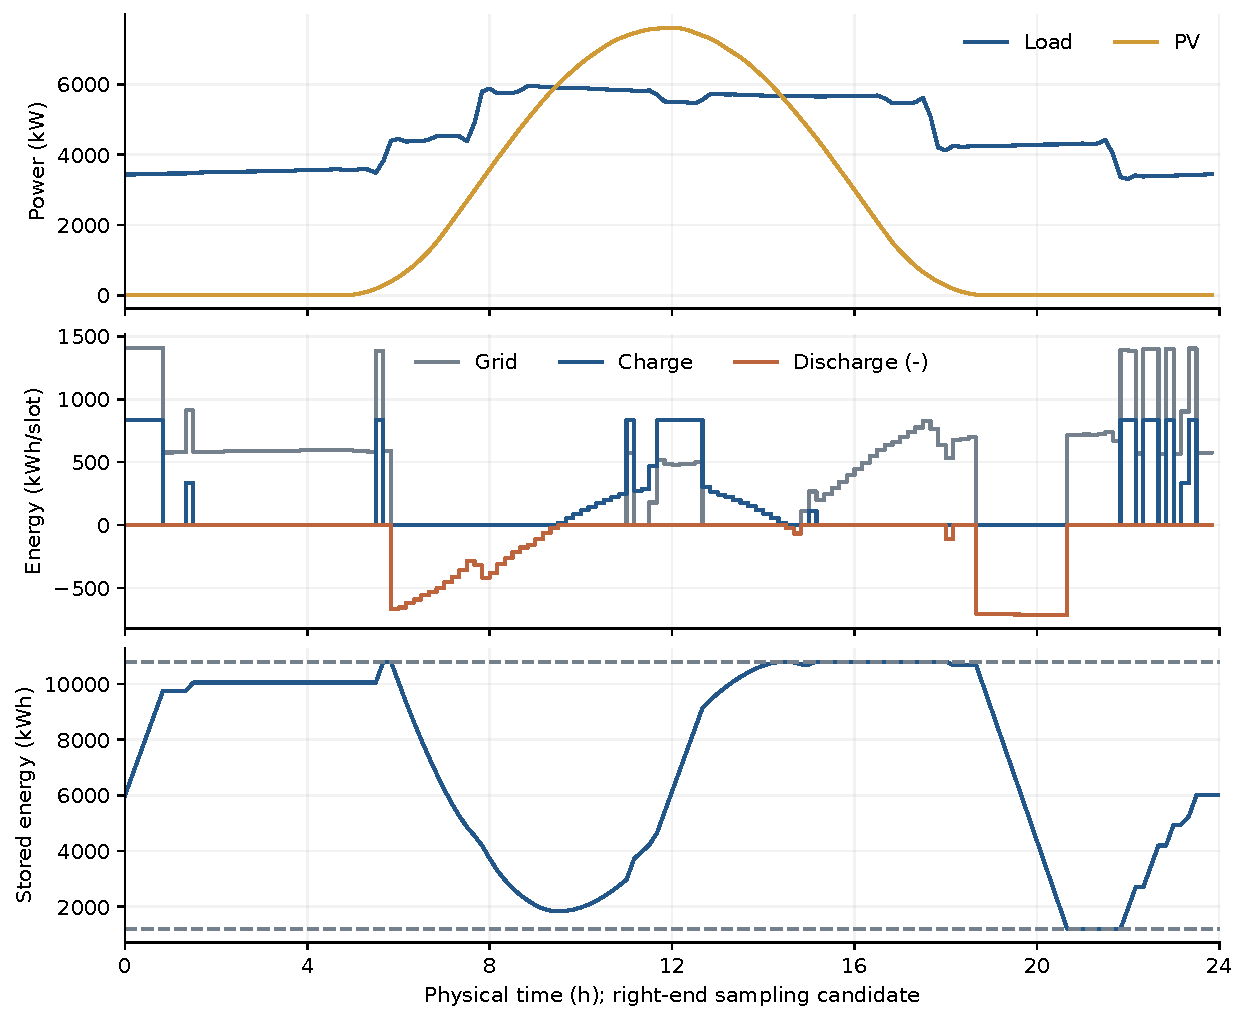
\includegraphics[width=.93\linewidth]{q1_dispatch.pdf}\caption{第一问优化调度。电量曲线按物理槽首绘制，储电量按区间边界绘制；放电以负值表示方向。}\label{fig:q1}\end{figure}
\begin{table}[H]\centering\caption{第一问指定物理时段的购电与充放电（候选）}\small
\begin{tabular}{lr}
\toprule
物理时段 & 购电量/kWh \\
\midrule
10:00--10:10 & 0.000 \\
12:00--12:10 & 480.412 \\
14:00--14:10 & 0.000 \\
16:00--16:10 & 445.432 \\
18:00--18:10 & 531.894 \\
20:00--20:10 & 0.000 \\
\bottomrule
\end{tabular}
\quad\begin{tabular}{lrr}
\toprule
物理时段 & 充电量/kWh & 放电量/kWh \\
\midrule
00:00--04:00 & 4500.000 & 0.000 \\
04:00--08:00 & 833.333 & 6365.841 \\
08:00--12:00 & 4787.964 & 1702.997 \\
12:00--16:00 & 5286.035 & 91.101 \\
16:00--20:00 & 0.000 & 5780.132 \\
20:00--24:00 & 5333.333 & 2859.868 \\
\bottomrule
\end{tabular}

\end{table}
日初和日末储电量均为6000 kWh。将90\%改为往返效率并对称分配到两个方向时，已有敏感性结果为33801.50元，比主口径低1325.45元；这是效率假设变化，不是算法节省。代表日附件没有真实日期，初始化日期仅作为程序锚点。

\section{第二问：成本敏感的安全裕量}
\subsection{预测残差与一月选型}
基础预测为$\widehat L_{d,t}=L_{d-7,t}$、$\widehat V_{d,t}=V_{d-1,t}$。历史净负荷残差记为
\begin{equation}
e_{d,t}=(L_{d,t}-V_{d,t})-(\widehat L_{d,t}-\widehat V_{d,t}).
\end{equation}
把一天分为6个四小时桶，在目标日前28日的已完成历史中，计算桶内原始残差分位数$q_{\tau,b}$；历史残差日不足7天时使用零裕量。修正预测为
\begin{equation}
\widetilde L_{d,t}=\widehat L_{d,t}+\kappa\max(0,q_{\tau,b(t)}),\qquad
\widetilde V_{d,t}=\widehat V_{d,t}.
\end{equation}
直接对原始残差求分位数，避免另加偏差项造成重复修正。候选包括零裕量及以下参数形成的八个组合：
\[\tau\in\{0.6,0.7,0.8,0.9\},\qquad\kappa\in\{0.5,1\}.\]
一月8日至14日建立残差历史，一月15日至31日比较完整实际成本，选择$\tau=0.8,\kappa=1$。二月起参数冻结，残差库仍只使用目标日前已经发生的数据。0.8是该候选网格的实测选择，不是由5倍价格在含储能情形下推导出的解析最优值。

\subsection{二乘二消融及费用分解}
B0和B1分别采用基础预测配合贪心控制与小时MPC；B2和B3在相同执行器上加入安全裕量。表\ref{tab:q2}中所有年度数字覆盖相同334天。
\begin{table}[H]\centering\caption{第二问费用比较；Oracle仅为事后信息对照}\label{tab:q2}\small\begin{tabular}{lrrr}
\toprule
方案 & 计划费/元 & 紧急费/元 & 总费/元 \\
\midrule
B0 & 12,258,250.77 & 4,323,292.77 & 16,581,543.53 \\
B1 & 12,258,250.77 & 4,292,554.51 & 16,550,805.27 \\
B2 & 13,706,009.44 & 1,431,977.61 & 15,137,987.06 \\
B3 & 13,706,009.44 & 1,434,937.88 & 15,140,947.32 \\
fixedG\_oracle & 12,258,250.77 & 1,958,975.02 & 14,217,225.79 \\
full\_oracle & 12,245,046.92 & 0.00 & 12,245,046.92 \\
\bottomrule
\end{tabular}
\end{table}
\fig{margin_mechanism}{1}{安全裕量的证据链：一月分时残差、实际参数组合费用、因果历史裕量和费用瀑布图。山脊图仅描述一月8至31日残差，各组峰高分别归一化；红线为该描述样本的80\%分位，不是每天实际使用的固定裕量。参数热力图仅展示已运行组合，没有插值。}
B2相对B0节省1443556.47元，降幅8.7058\%。其正常计划费增加1447758.68元，但应急费减少2891315.15元，净效果为总费下降。应急电量为380769.33 kWh，无收益富余为3505784.13 kWh，高于B0约211万kWh的富余。安全裕量以更多承诺购电及富余换取昂贵缺口的减少，因此应以总费而非单独的应急费判断成败。

逐日成对比较中，B2有291日总费低于B0，43日更高；月内分布仍有负收益尾部，不能把全年降低解释为每一天均改善。

B1仅比B0低30738.26元，B3反而比B2高2960.27元。在冻结预测和既定结算机制下，重新求解并不必然增加有价值的信息，MPC还可能选择另一组预测最优、实际费用不同的动作。因此本文以B2为第二问当前主候选。
\fig{strategy_stability}{1}{第二问的逐日成对比较、月内节省分布、累计节省和应急费用尾部。小提琴图的横线为中位数；经验超越概率包含全部334天。收益分布用于稳定性诊断，不作独立样本显著性检验。}

\subsection{完美信息基准}
固定合同Oracle保持B0的$G$不变，仅允许储能提前知道整日实际路径；全信息Oracle还允许据实际路径选择日前$G$。两者保持相同效率、功率、SOC和日终条件。其费用分别为14217225.79和12245046.92元。B0与固定合同Oracle相差2364317.74元，提示固定承诺下存在调度信息空间；但该差额不保证能由因果算法实现。B2与全信息Oracle仍相差2892940.14元，不能据此声称尚有同等金额的可实现优化。

\fig{dispatch_mechanism}{1}{储能执行与应急形成机制。上方与左下方采用题面指定的6月21日，右下方统计334天中每月各槽的日均应急电量；含零应急日。可达区域仅由SOC、功率与日终目标推导，不代表预测无误差。四个指定日明细仍见附录。}

\section{第三问：合同更新及价值门控}
\subsection{预报积分与逐次合同结算}
每次发布的未来24小时光伏预报按发布时间索引，仅在发布后使用。对整点功率作分段线性插值并积分到10分钟电量；从发布时刻到首个整点的缺失起点采用第一条预报保持的候选边界处理。后续发布仅截取当天剩余区间，不能改写已执行槽。

设一次更新前后合同为$G^{old},G^{new}$，定义$\Delta G^+=[G^{new}-G^{old}]_+$、$\Delta G^-=[G^{old}-G^{new}]_+$。采用“原合同退款后收50\%违约费”的候选解释，增量账本为
\begin{equation}
J^{adj}_k=\sum_{t\ge k}p_t(1.5\Delta G_t^+-0.5\Delta G_t^-),\qquad
J_3=\sum_t p_tG_t^{0}+\sum_kJ^{adj}_k+\sum_t5p_tU_t.
\end{equation}
每次均相对当前合同计算，不能反复相对零点合同收取费用。若题意采用取消部分不退款、另收违约费，则应另作敏感性，不可与上述费用混用。

\subsection{固定更新的实测结果}
对无裕量和有裕量各比较零点固定、旧PV重规划和新PV重规划。旧PV组在严格控制下没有实质合同调整，其总费仅与零点组存在数值舍入差。新PV组则包含实际合同变化。
\begin{table}[H]\centering\caption{第三问334天费用分解（万元）；旧PV组与对应固定组数值相同，正文不重复列示}\small\begin{tabular}{lrrrr}
\toprule
方案 & 计划费/万元 & 调整费/万元 & 紧急费/万元 & 总费/万元 \\
\midrule
基线固定 & 1231.6402 & 0.0000 & 408.6698 & 1640.3101 \\
基线更新 & 1231.6402 & 40.1133 & 383.0000 & 1654.7535 \\
裕量固定 & 1378.3454 & 0.0000 & 134.6222 & 1512.9676 \\
裕量更新 & 1378.3454 & 43.7750 & 146.2228 & 1568.3432 \\
裕量门控 & 1378.3454 & 22.0776 & 111.8091 & 1512.2321 \\
\bottomrule
\end{tabular}
\end{table}

裕量零点固定费用15129676.16元，低于无裕量固定组1273424.41元。对裕量方案，每次使用新PV并重规划反而增加553755.87元。因而不能以“预报更新更频繁”直接推出费用下降。旧执行器的同槽实际反馈结果与这里的信息时序不同，本文不把其改善幅度用于严格因果模型的论证。

\subsection{预期净收益门控}
在6、12、18点比较保持当前合同和接受新合同两种策略。以此前28日中最近20个可用完整历史日构造负荷及PV的联合残差路径，保留同日变量相关性和日内时序。历史PV残差对应同一发布时间的预报；不逐时段独立抽样。场景数不足7个历史日时回退为不更新。

每条场景分别计算两候选策略在余日的应急费用；预演中合同保持固定到日末，不假定未来还会得到何种新预报。两候选使用共同场景降低比较噪声。令
\begin{equation}
\widehat V_{keep}=\frac1S\sum_s J^{emg}_{keep,s},\quad
\widehat V_{update}=J^{adj}_k+\frac1S\sum_sJ^{emg}_{update,s}.
\end{equation}
仅当$\widehat V_{keep}-\widehat V_{update}>\theta$时更新；过去费用为沉没项，调整费只计一次。实际运行到下次发布时再重新评估。阈值在一月15日至31日从禁用、0、100、500及1000元中选择，最终为500元。

接受更新按6、12、18点分别为83、97和3次。这个差异描述本策略在当前数据及计费解释下的选择，不足以断言18点预报普遍无价值。

门控接受183次更新，共评估1002次，总费用15122320.83元。其应急费降至1118091.02元，但增加220775.53元调整费，相对裕量固定净节省仅7355.33元，约0.0486\%。全年7个月改善、4个月变差，见图\ref{fig:gate}。当前论文保留裕量固定为简单主候选，同时如实报告门控是这些严格第三问实验中的较低实测费用；不能将简单方案称为数值最优。事后收益只用于解释，不参与当时决策。
\begin{figure}[H]\centering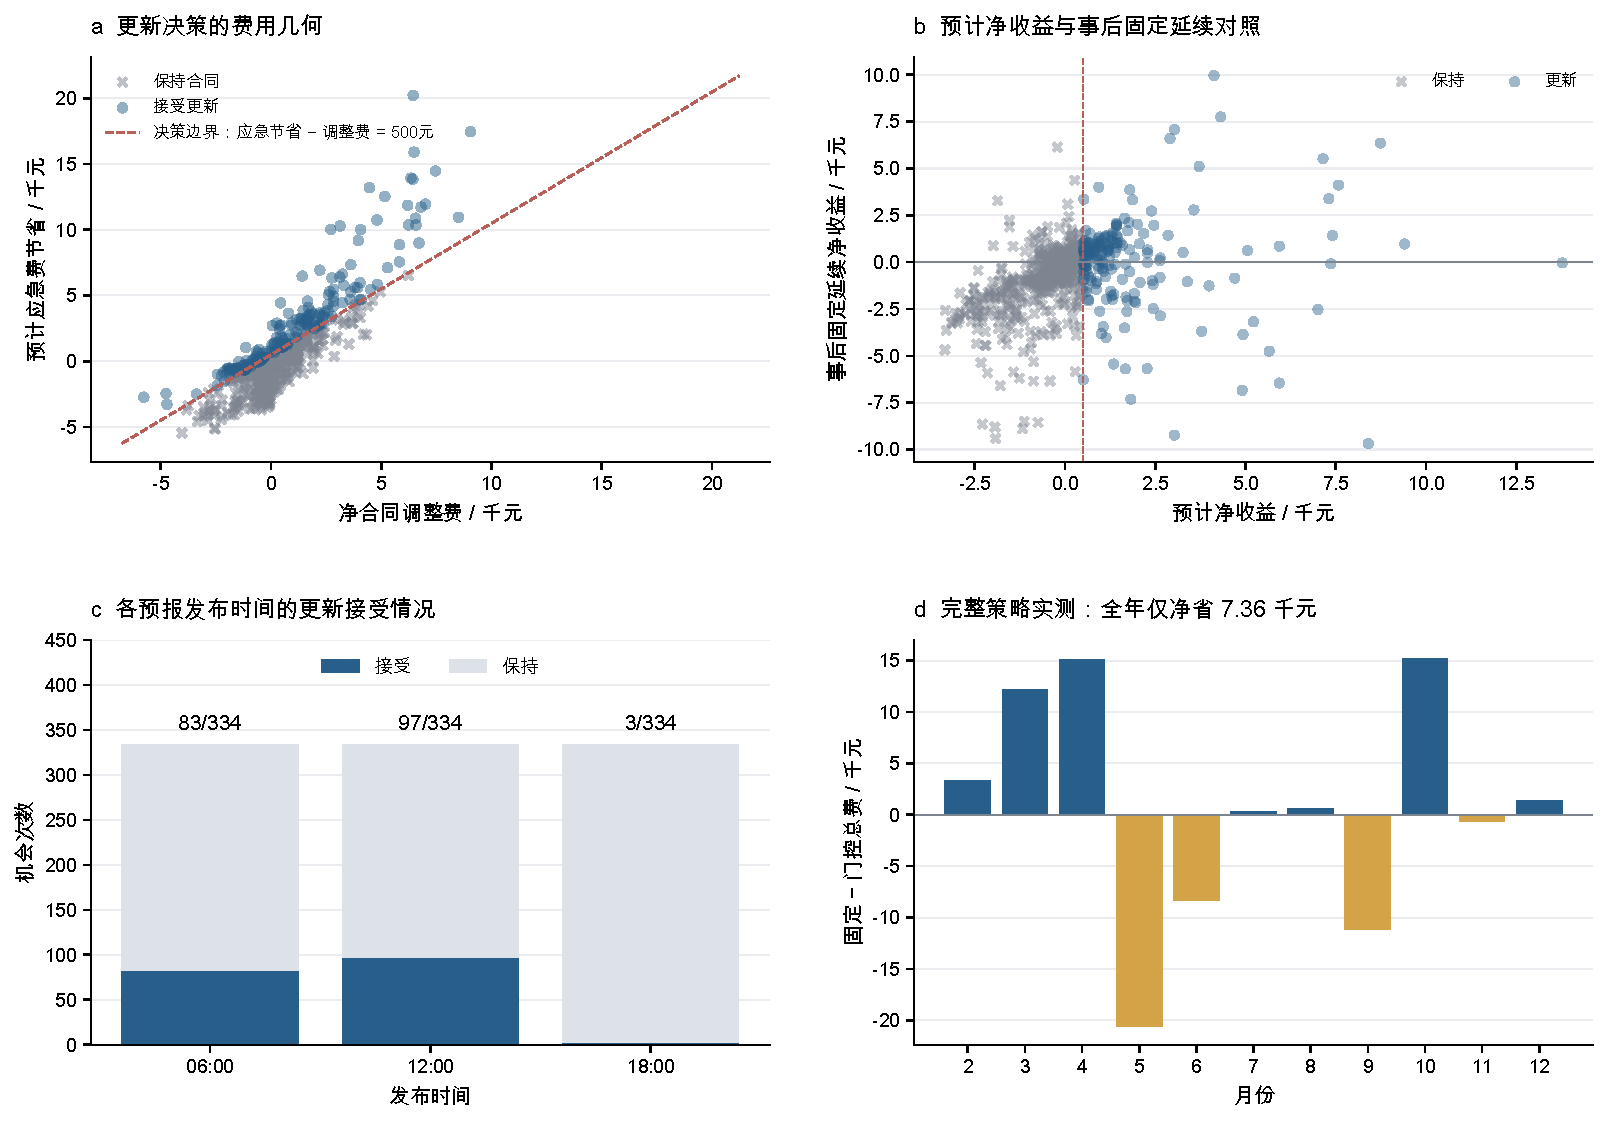
\includegraphics[width=\linewidth]{gate_decisions.pdf}\caption{第三问门控决策与回放检验。a中的净调整费可以为负；b是每次决策之后固定合同延续至日末的事后反事实，多个预演时域重叠，不能将其收益相加。d为完整运行策略的真实月度总费差，负值表示门控增费。}\label{fig:gate}\end{figure}

\section{第四问：动态电价下的迁移模型}
以$p_{d,t}$替换固定价格$p_t$，物理约束保持不变。日前策略最小化预测计划购电费，实际应急按$5p_{d,t}$结算；日内调整按$1.5p_{d,t}\Delta G^+-0.5p_{d,t}\Delta G^-$记账。价格输入必须同时用于计划、重规划、预演和实际账本，不能仅对第二、三问已有动作重新计价便声称完成重优化。

现有第四问实验采用“目标日整条价格曲线在零点可知”的条件假设。若只能知道当前或历史价格，则需另构造价格预测及信息集；费用变化应作为价格可知性敏感性。当前旧执行口径下，第四问日前与滚动候选费用分别为16233760.01元和14597113.33元，但其允许同槽实际总量参与储能反馈，\textbf{不能与本文第二、三问严格控制结果直接比较}。本稿仅将其列为历史记录，不填充为新版结论。

统一口径的第四问收尾需复用已选安全裕量和严格执行器，替换价格输入后重新求解、结算与独立复核。本稿没有声称该实验已经完成，也不以旧费用计算新增算法的节省率。

\section{校验、敏感性与模型局限}
\subsection{已有校验的含义}
现有独立验收文件记录了能量平衡、状态递推、功率及SOC边界、初末状态、互斥和费用复算。第二问B2独立物理残差最大为$4.55\times10^{-13}$ kWh，明显小于$10^{-6}$ kWh容差。控制重放以零值替换目标日实际序列，验证此前指令和合同不随未知实际值改变；第三问还检查发布时间、过去合同不可修改和逐次账本。

结果文件生成时可能保留“待独立验收”状态，实际验收应读取绑定结果的独立验证文件，而非仅看主文件状态字符串。该验证证明程序满足既定候选假设，并不证明候选解释即题面唯一解释。数值可行也不等于已通过最终模板及论文人工验收。

\subsection{解释边界}
\begin{enumerate}
\item 时间采样近似与模板区间尚待统一。右端矩形、左端矩形和梯形积分是不同假设，不能只改标签而保留全部费用结论。
\item 每日6000 kWh的终端要求是第二至四问主动采用的候选限制。放宽为跨日连续可能改变成本，不能归为算法创新收益。
\item 效率方向、母线侧功率、第三问减购退款、第四问价格已知性均需在最终正文与Excel说明保持一致。
\item 历史分位数与联合残差场景依赖误差的可迁移性；极端天气和负荷变化仍可能造成大量应急。当前没有验证全年真正分布外的泛化性能。
\item 槽末平衡描述的是聚合电量。若需要刻画实时快速储能反馈，应增加更细粒度测量与执行模型，不能用10分钟最终总量模拟无延迟控制。
\end{enumerate}
没有实施的CVaR、鲁棒模型或时间口径敏感性不列作实验成果。若以后修改参数并观察二月至十二月结果，应记录为新一轮开发版本，而非重复宣称独立测试。

\section{结论}
在当前候选口径下，统一物理模型可描述四问的共性，严格信息时序能明确区分规划与实际结算。第二问历史残差安全裕量取得较一致的费用改善，其机制为增加较便宜的计划电量、减少5倍应急，而非将应急清零。第三问实测表明，新预报带来的应急变化必须足以覆盖合同调整成本；门控相对简单裕量方案的净收益很小，保留简单策略具有解释与实现优势。

第二版论文已形成模型、回放证据和指定日表格的连贯叙述。最终封版仍依赖时间语义统一、第四问严格迁移和五份结果Excel的同版本重导出；在这些步骤完成前，不将本稿标作可直接提交的最终论文。

\begin{thebibliography}{9}
\bibitem{problem} 全国大学生数学建模竞赛组委会. 2026年高教社杯全国大学生数学建模竞赛C题：微网与外部电网电力调控策略及附件1--5[Z]. 2026.
\end{thebibliography}
\noindent\textit{引用说明：第二版仅使用已读取题面与本项目计算证据。队友文献库尚有条目待核验，未整库引入；正式文献综述与算法来源需在下一版补齐。}

\appendix
\section{第二问四个指定日的候选明细}
本附录采用B2的内部物理时段；费用为计划与紧急之和。连续紧急槽按相邻区间合并，阈值为$10^{-6}$ kWh。表格由运行轨迹自动生成，尚不表示官方模板映射已完成。
\subsubsection*{2025-03-20}
\begin{center}\small\begin{tabular}{lr}
\toprule
时段 & 购电量/kWh \\
\midrule
10:00--10:10 & 0.000 \\
12:00--12:10 & 538.078 \\
14:00--14:10 & 0.000 \\
16:00--16:10 & 449.121 \\
18:00--18:10 & 717.524 \\
20:00--20:10 & 0.000 \\
\bottomrule
\end{tabular}
\quad\begin{tabular}{lrr}
\toprule
时段 & 充电量/kWh & 放电量/kWh \\
\midrule
00:00--04:00 & 4500.000 & 0.000 \\
04:00--08:00 & 833.333 & 4820.169 \\
08:00--12:00 & 6062.807 & 3819.831 \\
12:00--16:00 & 5278.798 & 546.700 \\
16:00--20:00 & 0.000 & 5655.091 \\
20:00--24:00 & 5333.333 & 2984.908 \\
\bottomrule
\end{tabular}
\end{center}
全天计划购电量 69403.586 kWh，总费用 47,213.32 元，其中紧急费 4,830.84 元；日初、日末储电量均为6000 kWh。
\begin{longtable}{lr}\toprule 紧急购电物理时段 & 电量/kWh\\\midrule\endhead
00:20--00:30 & 10.820 \\
01:00--01:40 & 113.352 \\
03:10--03:30 & 45.273 \\
03:40--04:00 & 10.987 \\
09:50--10:00 & 16.348 \\
11:00--11:40 & 267.483 \\
12:20--13:40 & 565.833 \\
15:30--17:00 & 404.069 \\
17:20--17:30 & 6.655 \\
18:40--19:00 & 30.131 \\
21:10--21:40 & 9.856 \\
23:30--23:50 & 3.640 \\
\bottomrule\end{longtable}
\subsubsection*{2025-06-21}
\begin{center}\small\begin{tabular}{lr}
\toprule
时段 & 购电量/kWh \\
\midrule
10:00--10:10 & 0.000 \\
12:00--12:10 & 0.000 \\
14:00--14:10 & 0.000 \\
16:00--16:10 & 195.842 \\
18:00--18:10 & 220.356 \\
20:00--20:10 & 0.000 \\
\bottomrule
\end{tabular}
\quad\begin{tabular}{lrr}
\toprule
时段 & 充电量/kWh & 放电量/kWh \\
\midrule
00:00--04:00 & 0.000 & 0.000 \\
04:00--08:00 & 418.971 & 4320.000 \\
08:00--12:00 & 6904.691 & 0.000 \\
12:00--16:00 & 3343.004 & 0.000 \\
16:00--20:00 & 0.000 & 5781.027 \\
20:00--24:00 & 5333.333 & 2858.973 \\
\bottomrule
\end{tabular}
\end{center}
全天计划购电量 39985.338 kWh，总费用 24,257.70 元，其中紧急费 527.25 元；日初、日末储电量均为6000 kWh。
\begin{longtable}{lr}\toprule 紧急购电物理时段 & 电量/kWh\\\midrule\endhead
01:20--01:30 & 4.811 \\
01:50--02:00 & 5.781 \\
04:00--04:10 & 1.894 \\
05:50--06:20 & 24.340 \\
07:10--07:50 & 95.962 \\
09:00--09:10 & 5.668 \\
\bottomrule\end{longtable}
\subsubsection*{2025-09-23}
\begin{center}\small\begin{tabular}{lr}
\toprule
时段 & 购电量/kWh \\
\midrule
10:00--10:10 & 0.000 \\
12:00--12:10 & 495.788 \\
14:00--14:10 & 0.000 \\
16:00--16:10 & 571.697 \\
18:00--18:10 & 787.811 \\
20:00--20:10 & 0.000 \\
\bottomrule
\end{tabular}
\quad\begin{tabular}{lrr}
\toprule
时段 & 充电量/kWh & 放电量/kWh \\
\midrule
00:00--04:00 & 4500.000 & 0.000 \\
04:00--08:00 & 833.333 & 6014.927 \\
08:00--12:00 & 5873.974 & 2625.073 \\
12:00--16:00 & 5114.639 & 260.776 \\
16:00--20:00 & 0.000 & 5784.185 \\
20:00--24:00 & 5333.333 & 2855.815 \\
\bottomrule
\end{tabular}
\end{center}
全天计划购电量 71761.883 kWh，总费用 48,209.42 元，其中紧急费 3,641.20 元；日初、日末储电量均为6000 kWh。
\begin{longtable}{lr}\toprule 紧急购电物理时段 & 电量/kWh\\\midrule\endhead
00:40--00:50 & 18.879 \\
02:00--02:20 & 23.198 \\
05:00--05:10 & 11.088 \\
06:50--07:10 & 19.695 \\
07:50--08:00 & 3.058 \\
09:30--10:20 & 200.726 \\
10:40--11:00 & 10.011 \\
14:10--15:10 & 268.848 \\
16:00--16:10 & 17.736 \\
16:20--16:40 & 6.349 \\
18:10--18:30 & 33.963 \\
20:00--20:30 & 78.072 \\
20:50--21:10 & 54.838 \\
21:20--21:30 & 30.480 \\
22:20--22:30 & 14.773 \\
\bottomrule\end{longtable}
\subsubsection*{2025-12-21}
\begin{center}\small\begin{tabular}{lr}
\toprule
时段 & 购电量/kWh \\
\midrule
10:00--10:10 & 0.000 \\
12:00--12:10 & 958.629 \\
14:00--14:10 & 0.000 \\
16:00--16:10 & 805.047 \\
18:00--18:10 & 744.862 \\
20:00--20:10 & 0.000 \\
\bottomrule
\end{tabular}
\quad\begin{tabular}{lrr}
\toprule
时段 & 充电量/kWh & 放电量/kWh \\
\midrule
00:00--04:00 & 4500.000 & 0.000 \\
04:00--08:00 & 1666.667 & 1508.333 \\
08:00--12:00 & 5833.333 & 7806.667 \\
12:00--16:00 & 8333.333 & 2835.000 \\
16:00--20:00 & 0.000 & 5614.064 \\
20:00--24:00 & 5333.333 & 3025.936 \\
\bottomrule
\end{tabular}
\end{center}
全天计划购电量 101100.136 kWh，总费用 67,816.35 元，其中紧急费 2,416.92 元；日初、日末储电量均为6000 kWh。
\begin{longtable}{lr}\toprule 紧急购电物理时段 & 电量/kWh\\\midrule\endhead
03:00--03:10 & 13.363 \\
03:30--03:50 & 77.487 \\
10:20--11:30 & 564.551 \\
12:40--12:50 & 9.139 \\
18:20--19:00 & 54.040 \\
19:50--20:00 & 11.160 \\
22:50--23:00 & 1.635 \\
23:30--23:40 & 7.990 \\
\bottomrule\end{longtable}
\section{第三问四个指定日的候选明细}
本附录采用裕量零点固定主候选，因此调整量与原承诺相同、合同调整费为零。门控的较低全年实测成本已在正文另列，不能将两种策略拼接成一套提交结果。
\subsubsection*{2025-03-20}
\begin{center}\small\begin{tabular}{lr}
\toprule
时段 & 购电量/kWh \\
\midrule
10:00--10:10 & 0.000 \\
12:00--12:10 & 599.713 \\
14:00--14:10 & 0.000 \\
16:00--16:10 & 642.201 \\
18:00--18:10 & 717.524 \\
20:00--20:10 & 0.000 \\
\bottomrule
\end{tabular}
\quad\begin{tabular}{lrr}
\toprule
时段 & 充电量/kWh & 放电量/kWh \\
\midrule
00:00--04:00 & 4500.000 & 0.000 \\
04:00--08:00 & 833.333 & 5840.742 \\
08:00--12:00 & 6550.887 & 2799.258 \\
12:00--16:00 & 5945.791 & 1482.309 \\
16:00--20:00 & 0.000 & 5655.091 \\
20:00--24:00 & 5333.333 & 2984.908 \\
\bottomrule
\end{tabular}
\end{center}
全天计划购电量 73185.747 kWh，总费用 48,347.77 元，其中紧急费 3,565.06 元；日初、日末储电量均为6000 kWh。
\begin{longtable}{lr}\toprule 紧急购电物理时段 & 电量/kWh\\\midrule\endhead
00:20--00:30 & 10.820 \\
01:00--01:40 & 113.352 \\
03:10--03:30 & 45.273 \\
03:40--04:00 & 10.987 \\
08:10--08:30 & 57.907 \\
09:00--09:10 & 3.489 \\
09:40--11:40 & 704.563 \\
17:20--17:30 & 15.544 \\
18:40--19:00 & 30.061 \\
21:10--21:40 & 9.856 \\
23:30--23:50 & 3.640 \\
\bottomrule\end{longtable}
\subsubsection*{2025-06-21}
\begin{center}\small\begin{tabular}{lr}
\toprule
时段 & 购电量/kWh \\
\midrule
10:00--10:10 & 0.000 \\
12:00--12:10 & 0.000 \\
14:00--14:10 & 0.000 \\
16:00--16:10 & 224.337 \\
18:00--18:10 & 171.822 \\
20:00--20:10 & 0.000 \\
\bottomrule
\end{tabular}
\quad\begin{tabular}{lrr}
\toprule
时段 & 充电量/kWh & 放电量/kWh \\
\midrule
00:00--04:00 & 0.000 & 0.000 \\
04:00--08:00 & 97.885 & 4320.000 \\
08:00--12:00 & 7291.479 & 1.385 \\
12:00--16:00 & 3279.012 & 0.000 \\
16:00--20:00 & 0.000 & 5781.024 \\
20:00--24:00 & 5333.333 & 2858.976 \\
\bottomrule
\end{tabular}
\end{center}
全天计划购电量 39989.708 kWh，总费用 23,415.96 元，其中紧急费 27.02 元；日初、日末储电量均为6000 kWh。
\begin{longtable}{lr}\toprule 紧急购电物理时段 & 电量/kWh\\\midrule\endhead
01:20--01:30 & 4.811 \\
01:50--02:00 & 5.781 \\
04:00--04:10 & 1.939 \\
\bottomrule\end{longtable}
\subsubsection*{2025-09-23}
\begin{center}\small\begin{tabular}{lr}
\toprule
时段 & 购电量/kWh \\
\midrule
10:00--10:10 & 0.000 \\
12:00--12:10 & 438.775 \\
14:00--14:10 & 0.000 \\
16:00--16:10 & 595.756 \\
18:00--18:10 & 787.811 \\
20:00--20:10 & 0.000 \\
\bottomrule
\end{tabular}
\quad\begin{tabular}{lrr}
\toprule
时段 & 充电量/kWh & 放电量/kWh \\
\midrule
00:00--04:00 & 4500.000 & 0.000 \\
04:00--08:00 & 833.333 & 5058.319 \\
08:00--12:00 & 5833.333 & 3581.681 \\
12:00--16:00 & 5703.379 & 704.737 \\
16:00--20:00 & 0.000 & 5784.185 \\
20:00--24:00 & 5333.333 & 2855.815 \\
\bottomrule
\end{tabular}
\end{center}
全天计划购电量 75534.080 kWh，总费用 48,438.17 元，其中紧急费 1,276.88 元；日初、日末储电量均为6000 kWh。
\begin{longtable}{lr}\toprule 紧急购电物理时段 & 电量/kWh\\\midrule\endhead
00:40--00:50 & 18.879 \\
02:00--02:20 & 23.198 \\
05:00--05:10 & 11.020 \\
17:30--17:40 & 0.579 \\
18:10--18:30 & 32.933 \\
20:00--20:30 & 78.072 \\
20:50--21:10 & 54.838 \\
21:20--21:30 & 30.480 \\
22:20--22:30 & 14.773 \\
\bottomrule\end{longtable}
\subsubsection*{2025-12-21}
\begin{center}\small\begin{tabular}{lr}
\toprule
时段 & 购电量/kWh \\
\midrule
10:00--10:10 & 0.000 \\
12:00--12:10 & 1018.506 \\
14:00--14:10 & 0.000 \\
16:00--16:10 & 810.495 \\
18:00--18:10 & 744.862 \\
20:00--20:10 & 0.000 \\
\bottomrule
\end{tabular}
\quad\begin{tabular}{lrr}
\toprule
时段 & 充电量/kWh & 放电量/kWh \\
\midrule
00:00--04:00 & 4500.000 & 0.000 \\
04:00--08:00 & 1666.667 & 1508.333 \\
08:00--12:00 & 5833.333 & 7806.667 \\
12:00--16:00 & 7948.901 & 2523.610 \\
16:00--20:00 & 0.000 & 5614.064 \\
20:00--24:00 & 5333.333 & 3025.936 \\
\bottomrule
\end{tabular}
\end{center}
全天计划购电量 101377.694 kWh，总费用 66,217.94 元，其中紧急费 875.79 元；日初、日末储电量均为6000 kWh。
\begin{longtable}{lr}\toprule 紧急购电物理时段 & 电量/kWh\\\midrule\endhead
03:00--03:10 & 13.363 \\
03:30--03:50 & 77.487 \\
11:10--11:20 & 11.218 \\
12:40--13:10 & 19.223 \\
15:20--15:30 & 6.647 \\
16:20--16:30 & 13.682 \\
16:50--17:00 & 9.992 \\
18:20--19:00 & 54.039 \\
19:50--20:00 & 11.160 \\
22:50--23:00 & 1.635 \\
23:30--23:40 & 7.990 \\
\bottomrule\end{longtable}
\section{复现与交付索引}
模型代码位于项目\path{src/}，实验脚本位于\path{scripts/}；原始结果和独立验收位于\path{analysis/}。论文数值表由\path{scripts/paper/build_assets.py}生成，科研组图由\path{scripts/paper/build_research_figures.py}生成，输入文件摘要见候选图目录的\path{manifest.json}。

交付入口为\path{deliverables/README.md}；本稿源文件与PDF分别位于\path{draft_v2/latex/}、\path{draft_v2/pdf/}。候选图位于\path{candidate_figures/v2/}；旧五份Excel仅归档于\path{legacy_excel/}，与本文新策略不一致，不得混合作最终提交。正式提交目录在全部一致性验收后再填入最终产物。
\end{document}
